\section{Spectra of Graphs}

\subsection[Spectra -1]{1. Let $H_S$ be the hyperoctahedral graph obtained from the complete graph $K_{2s}$ by removing a perfect matching. Compute the spectrum of $H_2s$.}

The adjacency matrix of a perfect matching with $2s$ vertices can be written as a circulant matrix:
$$\text{circ}(0, \dots, 0, 1, 0, \dots, 0) \quad \text{ 1 at position $s+1$ }$$
just match vertices $1, \dots, s$ to vertices $s + 1, \dots, 2s$.

Hence the Hyperoctahedral graph (complementary of a perfect $2s$-matching has also a circulant adjacency matrix:
$$\text{circ}(0, 1, \dots, 1, 0, 1, \dots, 1) \quad \text{ 0s in position $0$ and $s + 1$ }$$
To compute it's eigenvalues we will use the known property of circulant graphs:
$$\lambda_k = \sum_{j=2}^n a_j \omega^{(j - 1)k} \quad \text{ where } \quad \omega = e^{\frac{2\pi i}{n}}$$

Now let us observe that:
\begin{itemize}
    \item If $k=0$: it is clear that $\lambda_0 = n -2$.
    \item If $k \neq 0$: substitute the coefficients $a_j$, and use that all the unit roots add to 0.
\end{itemize}

\subsection[Spectra - 2]{2. Show that the Petersen graph is the complement of the line graph of $K_5$. Compute the spectrum of the Petersen graph.}

\begin{definition}[Line Graph]
    Given a graph $G$, its line graph $L(G)$ is a graph such that:
    \begin{itemize}
        \item Each vertex of $L(G)$ represents an edge of $G$.
        \item Two vertices in $L(G)$ are adjacent if and only if their respective edges share a common endpoint in $G$.
    \end{itemize}
\end{definition}

Firstly, let us include a picture of the Petersen graph (which has 10 vertices and 15 edges):
\begin{figure}[h!]
    \centering
    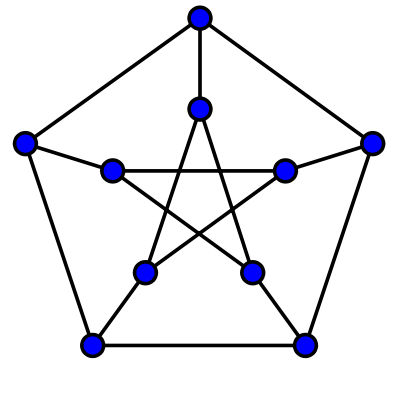
\includegraphics[width=.2\textwidth]{img/spectra_2.png}
\end{figure}

It is clear from the construction that $L(K_5)$ is 6-regular as each edge is incident to two vertices with three different incident edges each.
Further $L(K_5)$ has 10 vertices, and so does it's complementary.
Therefore it is clear that the complementary of the line graph is 3-regular with 10 vertices, hence it is the Petersen graph.

To compute its spectra, we will use the two following lemmas:
\begin{lemma}[Complement of a Graph]
    Let $G$ be an $r$-regular graph. Then,
    $$\phi(\bar{G}, x) = (-1)^n\left( \frac{x + r + 1 - n}{x + r + 1} \right) \phi(G, -x -1)$$
    where $\phi$ denotes the characteristic polynomial. 
\end{lemma}
\begin{lemma}[Line Graphs]
    Let $L(G)$ denote the line graph of $G$. Then if $G$ is $r$-regular,
    $$\phi(L(G), x) = (x + 2)^{m - n} \phi(G, x + 2 -r)$$
\end{lemma}
combining this two lemmas with the spectra of a graph with a circulant adjacency matrix ($K_5$) we can easily check the statement.

\subsection[Spectra - 3]{3. Check that $K_{10}$ contains two edge-disjoint copies of a Petersen graph. Show that $K_10$ does not contain three edge-disjoint copies of the Petersen graph.}

To see that it contains two edge-disjoint copies, it suffices to provide a drawing.
To see that it does not contain a third one, let us recall that the eigenvalues of the Petersen graph are $3$ with a multiplicity of 1, 1 with multiplicity of 5 and -2 with multiplicity of 4.
Let $A$ and $B$ be the adjacency matrix of the two edge-disjoint Petersen graphs, the remaining edge-disjoint graph $C$ would have an adjacency matrix:
$$C = 1_{10 \times 10} - I_{10 \times 10} - A - B$$
there exists $z \in V_A \cap V_B$ such that $z$ is orthogonal to 1, hence we have:
$$C z = (J - I - A - B)z = 0 = 0 - z - Az - Bz = -3z$$
and -3 is an eigenvalue of $C$ hence $C$ can not be a Petersen graph.

\subsection[Spectra - 4]{4. A graph $G$ is strongly regular with parameters $(n, r, \lambda, \mu)$ if it is a $r$-regular graph with $n$ vertices such that every two adjacent (non-adjacent) vertices have exactly $\lambda$ (resp. $\mu$) common neighbours. Show that the spectrum consists on 3 different graphs.}

First of all, the adjacency matrix of a regular graph is a matrix $A$ such that each row and column consists of exactly $r$ ones and $n-r$ zeros.
Then the square of that matrix has:
\begin{itemize}
    \item The main diagonal consisting in $r$'s: the number of walks of length 2 from a vertex to itself is their degree.
    \item Each row has $r$ $\lambda$s: the number of walks of length 2 between two adjacent vertices is, by definition, $\lambda$.
    \item The rest of the elements are $\mu$s.
\end{itemize}
Hence it can be expressed in the following way:
$$A^2 = rI + \lambda A + \mu(1_{n \times n} - I - A) = A^2 - (\lambda - \mu)A - (r - \mu)I - \mu V = 0$$
hence if $x$ is an eigenvalue of $A$, it must satisfy:
$$x^2 - (\lambda - \mu)x - (r - \mu) = 0$$

\subsection[Spectra - 5]{5. Let $G$ be a bipartite graph. (i) Show that the spectrum of $G$ is symmetric. (ii) Compute the spectrum of the bipartite complete graph $K_{r,s}$.}
